\documentclass{../../ExampleProblem}
\usepackage{../../mathshortcuts}
\usetikzlibrary{arrows}
\usepackage{stanli}

\usetikzlibrary{decorations.pathmorphing}
\usetikzlibrary{decorations.markings}


\title{Examples in TikZ}
\author{Brian Chevalier}
\subtitle{Drawing in TikZ}
\coursenum{GIT101}
\coursetitle{Intro to gitMechanics}
\university{gitMechanics}
\date{\today}



\begin{document}

\section{Basic Drawing Operations}

\subsection{Cartesian Coordinates}
\setcolumnwidth{6cm,2cm}
\begin{paracol}{2}
Drawing with the TikZ package must happen inside the TikZ environment. The simplest possible drawing is a straight line. Below is the code to draw a single line from (0,0) to (2,1). This line is drawn with cartesian coordinates. Note, the semicolon is necessary after each TikZ command or your document will not compile.

\centering
\begin{latexcode}
\draw (0,0) -- (2,1);
\end{latexcode}


\switchcolumn
\tikz \draw (0,0) -- (2,1);
\end{paracol}

\subsection{Polar Coordinates}
\begin{paracol}{2}
Here's how to draw with polar coordinates. The first number is the angle above the horizontal going counterclockwise, and the second number specifies the radius. The colon tells TikZ that the ordered pair is in polar coordinates and not cartesian.

\centering
\begin{latexcode}
\draw (0:2cm) -- (90:2cm);
\end{latexcode}


\switchcolumn
\tikz \draw (0:2cm) -- (90:2cm);
\end{paracol}


\subsection{Arbitrary Polygons}

\begin{paracol}{2}

You can connect multiple points in the same way but simply separating the points by double dashes. Notice the use of the keyword \textit{cycle}. This cycles the drawing back to the original point. This is the preferred way to enclose a polygon, rather than hardcoding in the original point again.

\centering
\begin{latexcode}
\draw (0,0) -- (1,0) -- (1,1) -- (0,1) -- cycle;
\end{latexcode}

\switchcolumn

\tikz \draw (0,0) -- (1,0) -- (1,1) -- (0,1) -- cycle;

\end{paracol}

\subsection{Relative Coordinates}

\begin{paracol}{2}
Sometimes you want to specify your next coordinate with the current coordinate as the origin of the next point.

Using a plus sign before the next specified point will place that point relative to the previous specified point. If you have multiple points in a row specified with a plus, the first point will be the origin relative to the following points.

Using two plus signs will \textit{always} use the previous point as the relative origin. The image at right shows the difference this makes.

\centering
\begin{latexcode}
\draw (0,0)--(1,0)--(1,1)--(0,1)--cycle;
\draw (1.25,0)--+(1,0)--+(1,1)--+(0,1)--cycle;
\draw (3,0)--++(1,0)--++(1,1)--++(0,1)--cycle;
\end{latexcode}

\switchcolumn

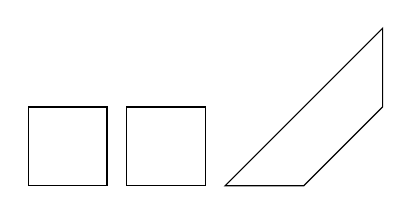
\begin{tikzpicture}
\draw (0,0)--(1,0)--(1,1)--(0,1)--cycle;
\draw (1.25,0)--+(1,0)--+(1,1)--+(0,1)--cycle;
\draw (2.5,0)--++(1,0)--++(1,1)--++(0,1)--cycle;
\end{tikzpicture}

\end{paracol}

\subsection{Shapes}


\begin{paracol}{2}
With very similar syntax, we can draw a simple rectangle by using the \textit{rectangle} keyword instead of two dashes. The first point indicates the bottom left corner of the rectangle, and the second point indicates the top right corner of the rectangle.

\centering
\begin{latexcode}
\draw (0,0) rectangle (2,1);
\end{latexcode}

\switchcolumn
\tikz \draw (0,0) rectangle (2,1);

\end{paracol}


\begin{paracol}{2}
We can draw a circle using the keyword \textit{circle}. The first point in parentheses is the center, the second number in parentheses is the radius.

\centering
\begin{latexcode}
\draw (0,0) circle (1cm);
\end{latexcode}

\switchcolumn

\tikz \draw (0,0) circle (1cm);

\end{paracol}


\begin{paracol}{2}
Drawing an ellipse is draw with the ellipse keyword. Just like circle the first coordinate is the center, the second argument is the x-radius and the y-radius separated from the keyword \textit{and}.

\centering
\begin{latexcode}
\draw (0,0) ellipse (2cm and 1cm);
\end{latexcode}

\switchcolumn

\tikz \draw (0,0) ellipse (2cm and 1cm);

\end{paracol}



\begin{paracol}{2}
Drawing an arc requires using the \textit{arc} keyword. The first number is the center of the arc (like the center of a circle or ellipse). The second set of information is the starting angle, ending angle, radius, separated by colons.

\centering
\begin{latexcode}
\draw (3,0) arc (0:90:2cm);
\end{latexcode}

\switchcolumn

\tikz \draw (3,0) arc (0:90:2cm);

\end{paracol}



\section{Styling Drawing Commands}
All of the drawing commands thus far have been basic thin lines, which are pretty boring. You can easily style drawings by giving the draw command optional arguments. There are many, many styles you can apply, so we're gonna try and focus on some basic ones and show you how to learn more.

Color, stroke width, line style, decoration


\subsection{Line Widths}

\begin{paracol}{2}

The following shows the different line widths you can use when drawing in TikZ. This should be an optional argument to the draw command. For instance, the first light, shown at right, is drawn with the following:

\centering
\begin{latexcode}
\draw[very thin] (0,0) -- (2,0);
\end{latexcode}
\switchcolumn

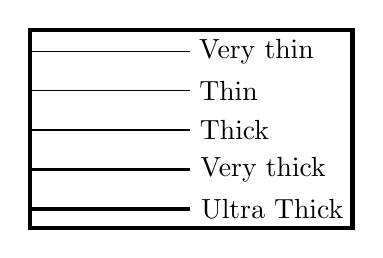
\begin{tikzpicture}[yscale=0.5]
\draw[very thin] (0,0) -- (2,0) node[right] {Very thin};
\draw[thin] (0,-1) -- (2,-1) node[right]{Thin};
\draw[thick] (0,-2) -- (2,-2) node[right]{Thick};
\draw[very thick] (0,-3) -- (2,-3) node[right]{Very thick};
\draw[ultra thick] (0,-4) -- (2,-4) node[right]{Ultra Thick};

\draw[ultra thick] (current bounding box.north east) rectangle (current bounding box.south west);

\end{tikzpicture}

\end{paracol}


\subsection{Line Types}

\begin{paracol}{2}

The example on the right shows different line styles you can use. Just like line widths you can use these as arguments to the draw command with the name in lowercase. The dashed line is drawn with: 

\centering
\begin{latexcode}
\draw[thick,dashed] (0,-1) -- (3,-1);
\end{latexcode}
\switchcolumn

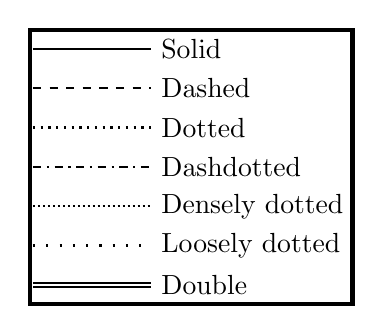
\begin{tikzpicture}[yscale=0.5,xscale=0.5]

\draw[thick,solid] (0,0) -- (3,0) node[right]{Solid};

\draw[thick,dashed] (0,-1) -- (3,-1) node[right]{Dashed};

\draw[thick,dotted] (0,-2) -- (3,-2) node[right]{Dotted};

\draw[thick,dashdotted] (0,-3) -- (3,-3) node[right] {Dashdotted};

\draw[thick,densely dotted] (0,-4) -- (3,-4) node[right] {Densely dotted};

\draw[thick,loosely dotted] (0,-5) -- (3,-5) node[right] {Loosely dotted};

\draw[thick,double] (0,-6) -- (3,-6) node[right] {Double};

\draw[ultra thick] (current bounding box.north east) rectangle (current bounding box.south west);
\end{tikzpicture}

\end{paracol}


\subsection{Filled Shapes}

\begin{paracol}{2}
Drawing a filled object is a matter of specifying a keyword argument, which is fill, with a value of the color you want. Using filldraw also allows setting the line color using the draw parameter.

\centering
\begin{latexcode}
\filldraw[fill=purple!20,
          draw=purple]
          (0,0) circle (1cm);
\end{latexcode}
\switchcolumn
\tikz \filldraw[fill=purple!20,draw=purple] (0,0) circle (1cm);

\end{paracol}

\subsection{Vertical Gradient}

\begin{paracol}{2}
Drawing an object with a gradient is done with the \textit{shadedraw} command instead of the draw command. Important note: the middle color should be specified last or it will not be recognized.

\centering
\begin{latexcode}
\shadedraw[top color=gray,
           bottom color=gray,
           middle color=white]
          (0,0) rectangle (2,1);
\end{latexcode}

\switchcolumn
\tikz \shadedraw[top color=gray, bottom color=gray,middle color=white] (0,0) rectangle (2,1);

\end{paracol}

\subsection{Horizontal Gradient}

\begin{paracol}{2}
Drawing an object with a gradient is done with the \textit{shadedraw} command instead of the draw command. Important note: the middle color should be specified last or it will not be recognized.

\centering
\begin{latexcode}
\shadedraw[left color=gray,
           right color=gray,
           middle color=white]
          (0,0) rectangle (2,1);
\end{latexcode}

\switchcolumn
\tikz \shadedraw[left color=gray,
           right color=gray,
           middle color=white]
          (0,0) rectangle (2,1);
\end{paracol}



\subsection{Radial Gradient}

\begin{paracol}{2}

\centering
\begin{latexcode}
\shadedraw[inner color=white,
           outer color=gray,
           draw=black]
           (0,0) circle (1cm);
\end{latexcode}

\switchcolumn

\tikz \shadedraw[inner color=white,
           outer color=gray,
           draw=black]
           (0,0) circle (1cm);

\end{paracol}










\section{Transformations}

\begin{paracol}{2}
Transformations can be applied to an entire tikzpicture, scope (discussed later), or a single command. There are many transformation options that can linearly transform the location of defined points.

\centering
\begin{latexcode}
\draw[step=0.1]
      0,0) grid (1.5,1);
\draw[cm={1.667,0.4,0.267,1.3,(0,0)},
      step=0.1] 
      (0,0) grid (1.5,1);
\end{latexcode}

The parameter \textit{cm} is the deformation map, while the second arguement coordinate pari of the x and y shift.

\switchcolumn

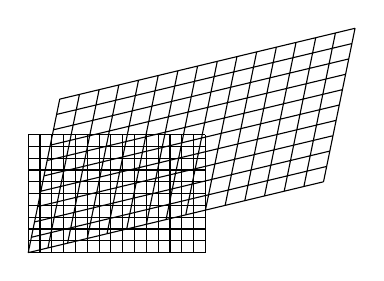
\begin{tikzpicture}[scale=1.5]
\draw[step=0.1] (0,0) grid (1.5,1);
\draw[cm={1.667,0.4,0.267,1.3,(0,0)},step=0.1] (0,0) grid (1.5,1);
\end{tikzpicture}

\end{paracol}




\section{Drawing with Scopes}

% Rotate around
% Scope trick.
% https://tex.stackexchange.com/questions/19284/problem-when-drawing-an-axis-aligned-bounding-box-around-a-tilted-rectangle

\begin{paracol}{2}

A scope is like a layer in Photoshop or AutoCAD. Scopes can have arbitrary options, the same options available when using the draw command, or optional inputs to a TikZ environment.



The figure shown at right shows how the idea of a \textit{scope} can be used to rotate objects in that scope about a point. The plate connected to the pin is drawn inside a scope environment.

The code to draw the rotated plate is shown below. The fist picture shows the final product. The second picture shows the plate at the original position before the \textit{rotate around} option is applied.

\begin{latexcode}
\begin{scope}[rotate around={-135:(0,0)}]
\draw[ultra thick,fill=lightgray]
      (0,0) rectangle (2,2);
\end{scope}
\end{latexcode}

\switchcolumn

\centering
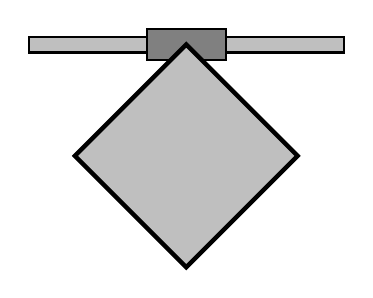
\begin{tikzpicture}[scale=1.0]

\shadedraw[top color=lightgray,middle color=gray,bottom color=lightgray,thick] (-2,-0.1) rectangle (2,0.1);
\draw[thick,fill=gray] (-0.5,-0.2) rectangle (0.5,0.2);

\begin{scope}[rotate around={-135:(0,0)}]
\draw[ultra thick,fill=lightgray] (0,0) rectangle (2,2);
\end{scope}
\poi{0,0}
%\poi{2,2}

\end{tikzpicture}

\vspace{0.5cm}

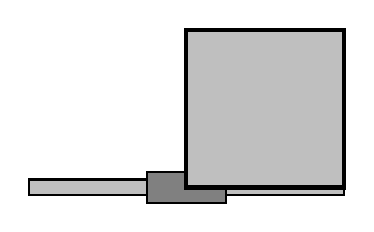
\begin{tikzpicture}[scale=1.0]

\shadedraw[top color=lightgray,middle color=gray,bottom color=lightgray,thick] (-2,-0.1) rectangle (2,0.1);
\draw[thick,fill=gray] (-0.5,-0.2) rectangle (0.5,0.2);

\begin{scope}[rotate around={0:(0,0)}]
\draw[ultra thick,fill=lightgray] (0,0) rectangle (2,2);
\end{scope}
\poi{0,0}
\poi{2,2}

\end{tikzpicture}

\end{paracol}

Figure \ref{Fig:mulispringsys} is a multi-spring system drawn with TikZ. The springs are rendered using the \textit{stanli} package. The package offers a spring lifestyle.

% https://tex.stackexchange.com/questions/430943/latex-stanli-package-how-to-design-a-spring-element#430951
\begin{figure}[H]
\centering
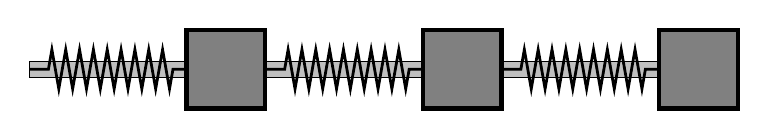
\begin{tikzpicture}

\draw[thin,fill=lightgray] (0,-0.1) rectangle (9,0.1);

\begin{scope}
\draw[ultra thick,fill=gray] (2,-0.5) rectangle (3,0.5);
\draw[spring] (0,0) -- (2,0);
\end{scope}

\begin{scope}[xshift=3cm]
\draw[ultra thick,fill=gray] (2,-0.5) rectangle (3,0.5);
\draw[spring] (0,0) -- (2,0);
\end{scope}

\begin{scope}[xshift=6cm]
\draw[ultra thick,fill=gray] (2,-0.5) rectangle (3,0.5);
\draw[spring] (0,0) -- (2,0);
\end{scope}

%\filldraw[shading=axis,top color=gray, bottom color=white,line width=10pt, cap=round] (0,-1) --(2,-1);

\end{tikzpicture}
\caption{Drawing springs}
\label{Fig:mulispringsys}
\end{figure}



\end{document}

